\scanpage{23}
% Folio d'archive : 22. Texte imprimé visible en transparence : verso, scan 024.
d) On veut que pour deux sous-catégories pleines $A',A''$ de $A$
\unsure{de réunion $A$}, qui sont soit des cribles soit des cocribles,
de réunion $A$, d'intersection $A_0$, l'application
\deleted{$\operatorname{Hom}($}
\[
\mathcal H(A)\longrightarrow\mathcal H(A')\times_{\mathcal H(A_0)}\mathcal H(A'')
\]
soit loc. \uline{surjective} sur les flèches
(elle a des chances d'être bijective sur les objets\ldots) i.e. pour
$\unsure{\xi|\zeta},\eta\in\operatorname{Ob}\mathcal H(A)$, on veut
\[
\operatorname{Hom}(\unsure{\xi|\zeta},\eta)\longrightarrow
\operatorname{Hom}(\unsure{\xi|\zeta}',\eta')
\times_{\operatorname{Hom}(\unsure{\xi|\zeta}_0,\eta_0)}
\operatorname{Hom}(\unsure{\xi|\zeta}'',\eta'')
\]
\uuline{surjectif}.
\margin{\figure{\begin{tikzpicture}\node[draw,ellipse] {Hot 7};\end{tikzpicture}}}
\margin{\uline{NB} Car on a déjà
$A=A'\amalg_{A_0}A''$ dans $(\mathrm{Cat})$}

On l'utilisera dans le cas de
\figure{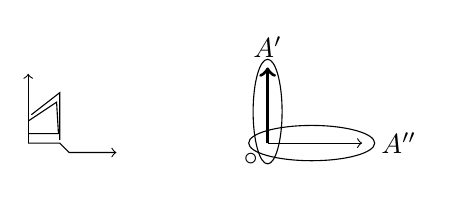
\begin{tikzpicture}[scale=.8]
\draw[->] (0,0)--(0,1.1);
\draw[->] (0,0)--(.5,0)--(.65,-.15)--(1.4,-.15);
\draw (0,.35)--(.45,.65)--(.48,.15)--(0,.15);
\draw (.05,.45)--(.5,.8)--(.5,.05);
\begin{scope}[xshift=3.8cm]
\node[below left] at (0,0) {$\circ$};
\draw[->,very thick] (0,0)--(0,1.2);
\draw[->] (0,0)--(1.5,0);
\node[above] at (0,1.2) {$A'$};
\node[right] at (1.65,0) {$A''$};
\draw (0,.5) ellipse (.23 and .83);
\draw (.7,0) ellipse (1 and .28);
\end{scope}
\end{tikzpicture}}
et le cas dual, et les produits par \unsure{tt élément|tout élément} $B$ de Cat
